\subsection{LatentMoE: Hardware-Aware Expert Design for Improved Accuracy per Byte}
\label{subsec:latentmoe}

\begin{figure}[h!tb]
    \centering
    \begin{subfigure}[b]{0.42\textwidth}
        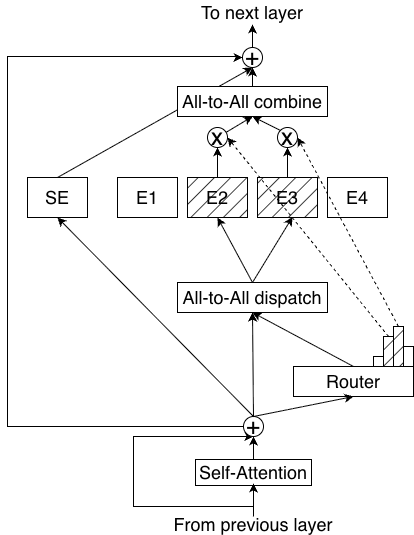
\includegraphics[width=\textwidth]{figures/standard_moe.png}
        \caption{Standard MoE architecture.}
        \label{fig:standard_moe}
    \end{subfigure}
    \hfill
    \begin{subfigure}[b]{0.45\textwidth}
        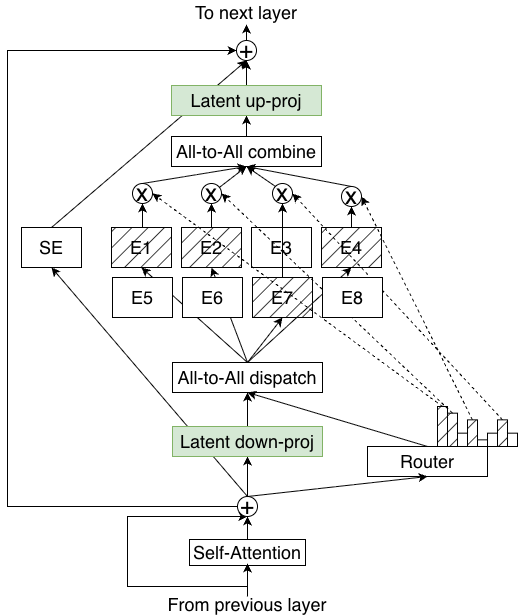
\includegraphics[width=\textwidth]{figures/latent_moe.png}
        \caption{LatentMoE architecture.}
        \label{fig:latent_moe}
    \end{subfigure}
    \caption{Standard MoE vs. LatentMoE architectures. In LatentMoE, tokens are projected from the model hidden dimension $d$ into a smaller latent dimension $\ell$ for expert routing and computation, which reduces routed parameter loads and all‑to‑all traffic by a factor of $d / \ell$ (typically about $4\times$). We use this efficiency to increase both the total number of experts and the top-$K$ active experts per token by the same factor $d/\ell$, which improves accuracy per byte while keeping overall inference cost approximately constant.}
\end{figure}

Transformer models are typically deployed in two distinct settings: latency-focused deployments that prioritize response time, and throughput-focused deployments that maximize token processing capacity.
Mixture of Experts (MoE) layers face fundamentally different performance bottlenecks depending on the scenario.
In latency-focused deployments, the model processes tens to hundreds of tokens at a time to minimize end-to-end latency. In this regime, MoE computation is memory-bandwidth-bound: reading expert weights from memory dominates the cost and far exceeds the actual computation time. Each expert matrix has size $d \times m$, where $d$ is the model hidden dimension and $m$ is the expert FFN intermediate dimension, so reducing memory bandwidth costs requires decreasing either $d$ or $m$.
In throughput-focused deployments, the model processes thousands of tokens per iteration to maximize throughput. In this regime, the all-to-all communication required to dispatch tokens to experts and aggregate results emerges as the primary bottleneck. The communication volume scales linearly with the number of top-$K$ active experts $K$ and the hidden dimension $d$, but is independent of the expert FFN intermediate dimension $m$.
At the same time, the expressive power of FFN layers is primarily controlled by the effective nonlinear budget, which is roughly proportional to $K \times m$.

Our objective is to improve model quality without compromising inference throughput or latency.
Guided by the above insights, we adopt a specific design choice. To improve accuracy per byte, we shrink the \emph{routed} expert input dimension $d$ to reduce communication and memory costs, and reinvest
the saved capacity into increasing the nonlinear budget and expert diversity by scaling up both the
total number of experts $N$ and the top-$K$ active experts per token. LatentMoE is a novel architecture that implements this strategy.

The LatentMoE architecture is illustrated in Figure~\ref{fig:latent_moe}. Each token embedding is first projected from the original hidden dimension $d$ into a latent representation of smaller dimension $\ell < d$, routed to an expanded set of experts that operate entirely in this latent space, and then projected back to the original hidden dimension $d$.
By shifting routed expert computation and all-to-all traffic to the latent space, both per-expert weight loads and communication payloads are reduced by a factor of $d / \ell$ compared to a standard MoE. 
We use these parameter and bandwidth savings to increase both the total number of experts from $N$ to $N' = N \cdot d / \ell$ and the top-$K$ active experts per token from
$K$ to $K' = K \cdot d / \ell$. The reduction in dimensionality offsets the increase in expert count and active experts, which enables higher model quality at similar computational and communication budget.
To preserve quality, all non-routed computations, including the MoE routing gate (gating network), shared expert computation, and non-expert layers, remain in the original hidden dimension $d$, since they do not significantly contribute to the targeted bottlenecks.

\begin{table}
    \centering
    \caption{Comparison of downstream task accuracy between Standard MoE and LatentMoE. The LatentMoE architecture consistently outperforms the standard MoE baseline across all evaluated tasks.}
    \label{tab:latent_moe_8B_1T_results}
    \begin{tabular}{c||c|c|c|c|c}
        \toprule
        \multirow{2}{*}{\textbf{Model}} & \multicolumn{5}{c}{\textbf{Accuracy (\%)}} \\
        \cline{2-6}
         & \textbf{MMLU-Pro} & \textbf{MMLU} & \textbf{Code} & \textbf{Math} & \textbf{\begin{tabular}{@{}c@{}}Commonsense\\Understanding\end{tabular}} \\
        \hline
        \begin{tabular}{@{}c@{}}\textbf{Standard MoE}\\(8.09B active / 72.6B total)\end{tabular} & 48.30 & 70.10 & 51.95 & 78.32 & 81.73 \\
        \hline
         \begin{tabular}{@{}c@{}}\textbf{LatentMoE}\\(8.02B active / 72.8B total)\end{tabular} & \textbf{52.87} & \textbf{72.11} & \textbf{55.14} & \textbf{80.19} & \textbf{82.10} \\
        \bottomrule
    \end{tabular}
\end{table}

Table~\ref{tab:latent_moe_8B_1T_results} compares the downstream performance of Standard MoE and LatentMoE. To provide a comprehensive evaluation, we report aggregated scores: ``Code'' averages HumanEval, HumanEval+, MBPP, and MBPP+; ``Math'' averages GSM8K CoT and MATH-500; and ``Commonsense Understanding'' averages RACE, ARC-Challenge, HellaSwag, and Winogrande. Both models feature 8 billion active and 73 billion total parameters, and were trained for 1 trillion tokens using identical hyperparameters. Specifically, the Standard MoE model uses a hidden dimension of size $d=4096$ and 128 total experts with 6 active experts, while LatentMoE uses a latent dimension $\ell=1024$ and 512 total experts with 22 active experts. As the results demonstrate, LatentMoE consistently outperforms the Standard MoE baseline across all evaluated tasks.